\clearpage
\chapter*{CFAR Staff}
\begin{longtable} { p{.3\textwidth} p{.7\textwidth} }

\raisebox{-.92\height}{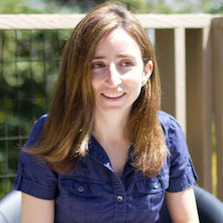
\includegraphics[width=4cm]{../../../img/headshots/anna.png}} & \textbf{Anna Salamon} likes finding analogies between human rationality and machine learning/artificial intelligence.  She also enjoys building implicit models of the human psyche by looking at how it expresses itself in the structure of religion and philosophy.  Finally, she loves to hear others' ideas on how to teach agency and epistemic integrity, especially ones that the current CFAR curriculum may have missed. \\
\\

\raisebox{-.92\height}{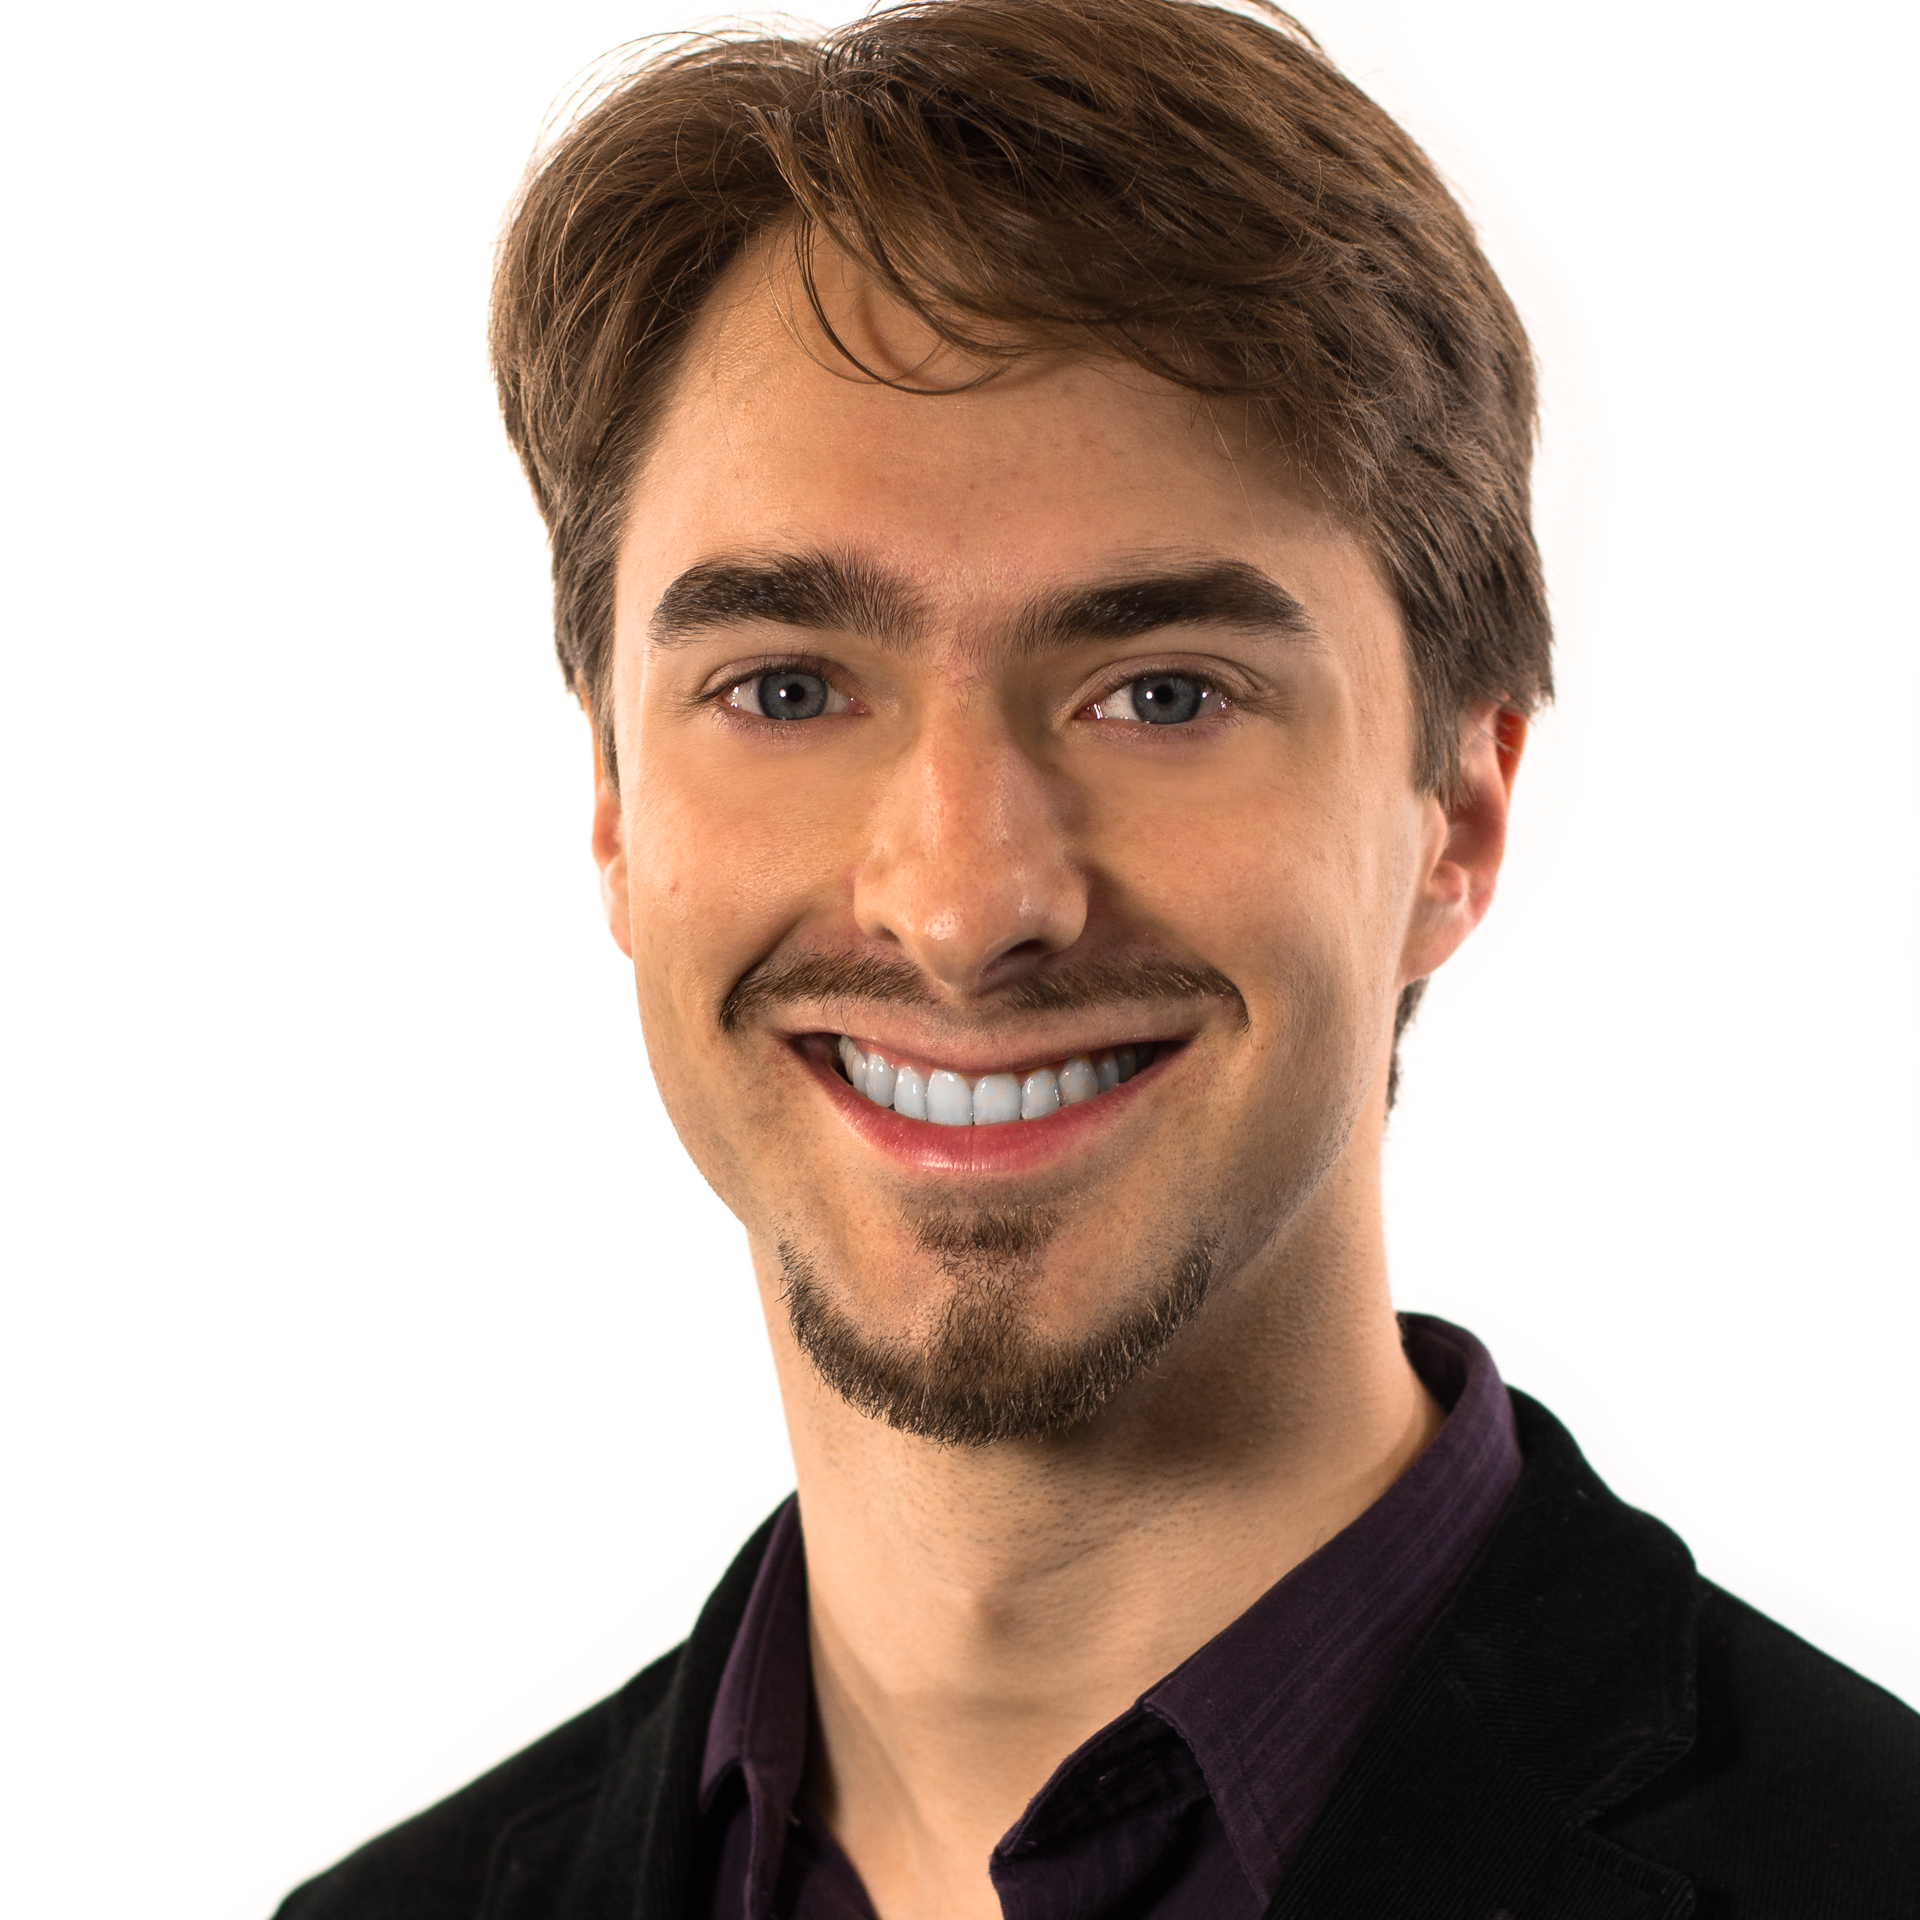
\includegraphics[width=4cm]{../../../img/headshots/val.png}} & \textbf{Val Smith} is interested in applying \emph{mindfulness} to rationality, which often means stripping out the mystical/transcendental talk and zeroing in on practical application and objective changes to thought process.  He has an MS in mathematics and a Ph.D. in math and science education research, and is skilled in the martial art of aikido. \\
\\

\raisebox{-.92\height}{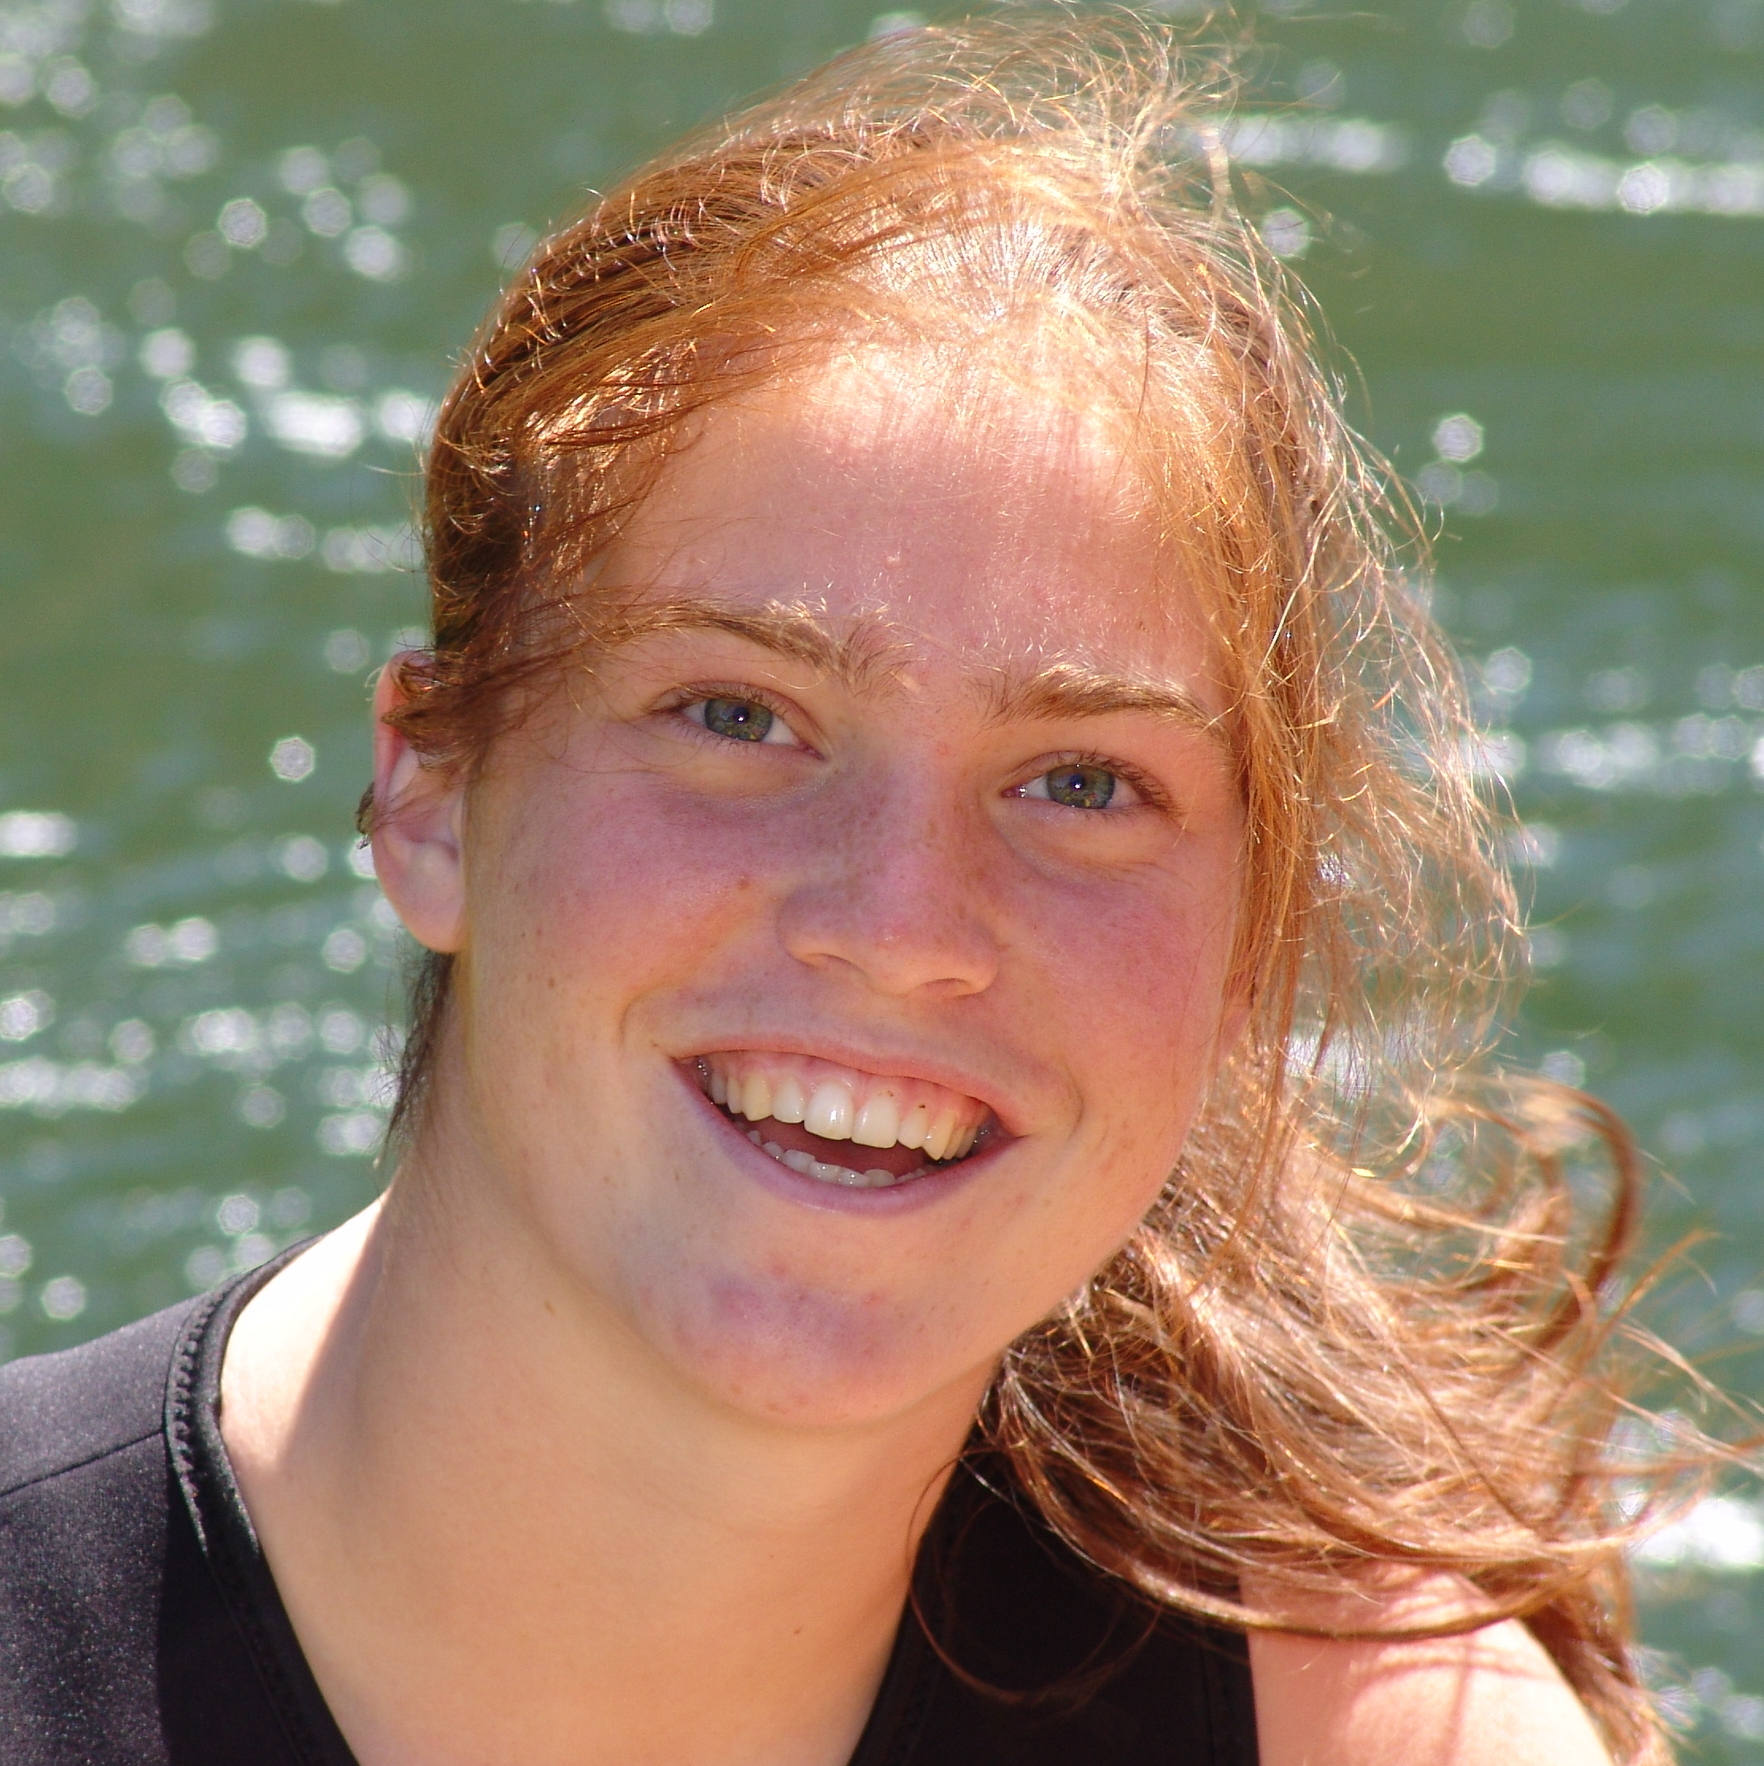
\includegraphics[width=4cm]{../../../img/headshots/kenzi.png}} & \textbf{Kenzi Amodei} is particularly interested in the relationship between rationality and emotion (how each can support, influence, or undermine the other).  Working with CFAR is Kenzi's third "career" \ldots she has a BA in Drama from Stanford University and a BS in General Science from the University of Oregon, and has worked as a professional stage manager and an undergraduate biology lab instructor.\\
\\

\raisebox{-.92\height}{
\includegraphics[width=4cm]{../../../img/headshots/duncan.png}} & \textbf{Duncan Sabien} wants to leave the universe noticeably different than it was before he arrived, and he's currently trying to do this through making things and teaching people.  He has a background in LEGOs, parkour, and middle grades education, and is easily manipulated by people quoting \underline{Ender's Game}. \\
\\

\raisebox{-.92\height}{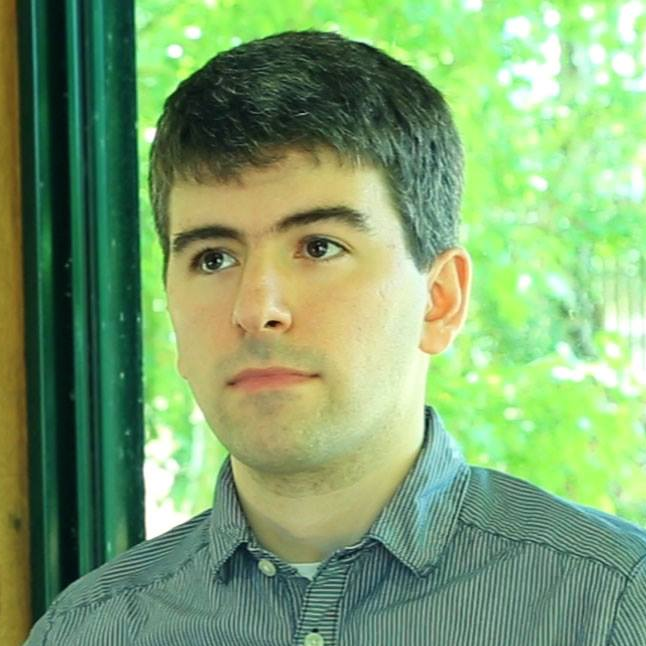
\includegraphics[width=4cm]{../../../img/headshots/dan.png}} & \textbf{Dan Keys} has a background in heuristics and biases research.  He is interested in finding measurable variables that help to reveal the effects of rationality training, and distinguish between various methods or approaches.  He's curious about which research projects CFAR should run in the future, as well as what kinds of studies academic researchers should be conducting, and what self-tracking individuals would find useful. \\
\\

\raisebox{-.92\height}{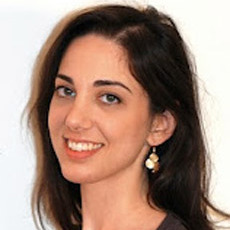
\includegraphics[width=4cm]{../../../img/headshots/julia.png}} & \textbf{Julia Galef} has a background in statistics, social science research, and economics, including writing case studies for the Harvard Business School.  Her recent career included several years in New York, where she wrote and gave lectures on science, philosophy, and design before moving to Berkeley to co-found CFAR.  In her spare time, she hosts the "Rationally Speaking" podcast, and loves talking about ethics, food, and scientific methodology. \\
\\

\raisebox{-.92\height}{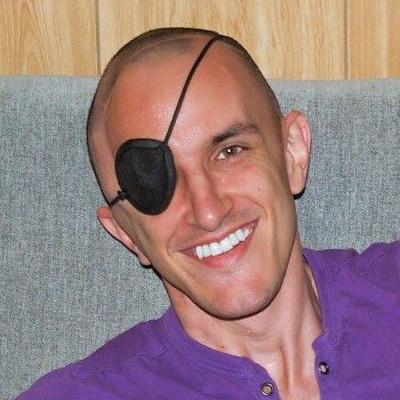
\includegraphics[width=4cm]{../../../img/headshots/pete.png}} & \textbf{Pete Michaud} has previously worked as a software developer, an architect, and a consultant.  He cofounded Connection Corps, an emotional intelligence education organization in Austin, Texas.  Before joining CFAR, he spent time helping the effective altruism movement get off the ground through EA Global and EA Action.\\
\\

\raisebox{-.92\height}{
\includegraphics[width=4cm]{../../../img/headshots/davis.png}} & \textbf{Davis Kingsley} likes rationality, Stoicism, and people with coherent and unusual life philosophies.  

\end{longtable}
\clearpage



